\documentclass[conference]{IEEEtran}
\usepackage[latin9]{inputenc}
\pagestyle{headings}
\usepackage{amsmath,amssymb}
\usepackage{graphicx,epsfig}
\usepackage{mathptmx,times} % if new font selection scheme installed
\usepackage{epstopdf}
\usepackage{tikz}
\usepackage[europeanresistors,americaninductors]{circuitikz}

\makeatletter
%%%%%%%%%%%%%%%%%%%%%%%%%%%%%% User specified LaTeX commands.
\hyphenation{op-tical net-works semi-conduc-tor}

\newcommand{\MYfooter}{\smash{
\hfil\parbox[t][\height][t]{\textwidth}{}\hfil\hbox{}}}

\def\ps@IEEEtitlepagestyle{%
\def\@oddhead{\mbox{}2016 ICSEE International Conference on the
     Science of Electrical Engineering \rightmark \hfil }%
\def\@oddfoot{\MYfooter}%
\def\@evenfoot{\MYfooter}}

% adjust as needed
\addtolength{\footskip}{0\baselineskip}
\addtolength{\textheight}{-1\baselineskip}

%%%%%%%%%%**********%%%%%%%%%%**********%%%%%%%%%%**********%%%%%%%%%%
\newtheorem{theorem}{Theorem}[section]
\newtheorem{corollary}[theorem]{Corollary}
\newtheorem{lemma}[theorem]{Lemma}

\newtheorem{proposition}[theorem]{Proposition}
\newtheorem{definition}[theorem]{Definition}
\newtheorem{example}[theorem]{Example}
\newtheorem{problem_statement}[theorem]{Problem Statement}
\newtheorem{remark}[theorem]{Remark}
%\numberwithin{equation}{section}
%%% The above 7 commands are used in the following way:
%%% The definition environment, for example, is created by
%%% \begin{definition}\label{xxx}. . .\end{definition}
%\newcommand{\mylabel}[1]{\label{#1}
%            \ifx\undefined\stillediting
%            \else \fbox{$#1$}\fi }
\newcommand{\BE}{\begin{equation}}
\newcommand{\BEQ}[1]{\BE\label{#1}} % Changed by Olof
\newcommand{\EEQ}{\end{equation}}
\newcommand{\rfb}[1]{\mbox{\rm
   (\ref{#1})}\ifx\undefined\stillediting\else:\fbox{$#1$}\fi}
\newenvironment{matr}[1]{\left[ \begin{array}{#1}}{\end{array}
                         \right]}
%
%\newfont{\roma}{cmr10 scaled 1200}
%\font\fourteenrm = cmr10  scaled\magstep2
%
\renewcommand{\cline}{{\mathbb C}}
\newcommand{\rline}  {{\mathbb R}}
\renewcommand{\l}    {{\lambda}}
\renewcommand{\o}    {{\omega}}
\newcommand{\e}      {{\varepsilon}}
\newcommand{\half}   {{\frac{1}{2}}}
\newcommand{\m}      {{\hbox{\hskip 1pt}}}
\newcommand{\nm}     {{\hbox{\hskip -3pt}}}
\newcommand{\dd}     {{\rm d\hbox{\hskip 0.5pt}}}

\makeatother

%%%%%%%%%%**********%%%%%%%%%%**********%%%%%%%%%%**********%%%%%%%%%%
\begin{document}

\title{ Exponential stability  of a microgid comprising of two identical synchronous generators}
\author{\IEEEauthorblockN{Elad Venezian} \IEEEauthorblockA{School of 
   EE, Tel Aviv University\\ Ramat Aviv 69978, Israel} \and 
   \IEEEauthorblockN{George Weiss} \IEEEauthorblockA{School of EE, 
   Tel Aviv University\\ Ramat Aviv 69978, Israel}}

\maketitle

\begin{abstract}
Synchronous generators are an essential component of the electric
grid. Recently, the stability of the electric grid has become an area
of high interest and intensive research. We discuss the stability of a
grid composed of two identical synchronous generators, and show sufficient conditions for exponential stability.
\end{abstract}

%%%%%%%%%%**********%%%%%%%%%%**********%%%%%%%%%%**********%%%%%%%%%%
\section{Introduction}

The AC electricity grid was developed at the end of the XIXth century,
and has remained very similar until today. The grid is an enormously
complex nonlinear and randomly varying system for which rigorous
stability analysis is impossible. Many techniques and models that have
been developed to assess the stability of a power grid, using rigorous
modelling and system theory techniques mixed with practical shortcuts
and simplifying assumptions driven by experience, see for instance
\cite{Kundur}, \cite{GrSt2014}, \cite{SauerPai1998}, \cite{GOBS:03},
\cite{DoBull:12}.

In recent years, due to the increasing penetration of renewable energy
resources, which connect to the grid via power converters and produce
an intermittent power output, it is not clear whether the traditional
models and methods for controlling the power grid will succeed to
control it. Therefore, there is an increasing interest in the
fundamental mathematical models and stability analysis for the grid,
see for instance \cite{DoBull:12}, \cite{PoDoBu:13}, \cite{CaTa:14},
\cite{NaWe:14}, \cite{NaWe:15}, \cite{DePersiSchaft:16}.

The {\em synchronous generator} (SG) is the main power source of the
electricity grid. The mathematical model of a SG (see the earlier
references and in addition \cite{Walker:94}, \cite{Fitzgerald:03},
\cite{MaWe:15}, etc.) is complex and difficult to use as a component
when we model a large network. Stability analysis is usually done
either by simulation, or analytically on simplified models, in which
the SGs are connected in a simple network and each SG is represented
by reduced order equations, see for instance \cite{DoBull:12} and
\cite{PoDoBu:13}. The reduced model of a SG is often obtained by
treating the stator currents as fast variables, thus eliminating them
from the state variables via the singular perturbation approach (see,
for instance, \cite{Khalil}) and keeping only the rotor angle, the
rotor angular velocity and the rotor field as relevant state
variables, see for instance \cite{Kundur} and \cite{SauerPai1998}.

SGs have the important property that once they synchronize, they tend
to remain synchronized even without any control. This is important
attribute because the electricity grid must maintain nearly constant
frequency, and because the ability of a SG to transfer constant power
to the grid exists only when the phase difference between it and the
grid is constant. Therefore, it is desirable to know if for a given
grid which contains SGs and a loads, the SGs tend to synchronize (for
initial states in a reasonably large region) and if yes, if the grid
frequency and power flows remains stable. To simplify the stability
analysis, it is common to use the Park transformation of the voltages
and currents, that maps sinusoidal positive sequence signals into a
fixed point in the state space.

In this paper, we study the configuration of a two identical SGs in parallel and a resistive  load. 

The rest of this paper is organized as follows. In Section II, a
fourth order model of a SG connected to infinite bus and having
constant field current is presented. The model of {\em two identical coupled SGs} (TICSG) is described in Section III. In section IV, we discuss  the equilibrium points of the TICSG system.
Stability analysis for the TICSG is given in Section IV.

%%%%%%%%%%**********%%%%%%%%%%**********%%%%%%%%%%**********%%%%%%%%%%
\section{Modeling SG connected to infinite bus}

In this section we derive the equations for a SG connected to infinite
bus and having a constant field (or rotor) current. We start with
deriving the equations for single SG, assuming constant field current,
following the notation in \cite{ZhWe:11}. 

The rotor of a SG is a winding (coil) on a magnetic core that spins
inside a circular cavity in the stator, having an angle $\theta$ with
respect to a reference angle, see Figure 1. We denote its self
inductance by $L_f$, its resistance by $R_f$, the voltage across its
terminals by $v_f$ and the current through it (called the field
current) by $i_f$. We assume for simplicity that $L_f$ is independent
of $\theta$ and $i_f$. The stator consists of three identical windings
that are connected in a star, with phase shifts of $120^0$ (see again
Figure 1). We consider that there is no neutral connection and no
damper windings. The stator windings can be regarded as connected
coils with self inductance $L$, mutual inductance $-M$, and resistance
$R_s$ (the parameters $L_f,R_f,L,M,R_s$ are positive). We assume no
magnetic saturation effects in the iron core and no Eddy currents. The
stator terminals are labeled with the letters $a,b,c$ and the vector
of voltages on the stator terminals is denoted by $v=\left[v_a\ v_b\
v_c\right]^\top$. We denote by $v_s$ the voltage at the unconnected 
center of the star (see Figure 1) and $v^n=[v_s\ v_s\ v_s]^\top$.
We define the vectors
$$ \widetilde{\cos}\m\theta \m=\m \left[\begin{array}{c} \cos\left(
   \theta\right)\\ \cos\left(\theta-\frac{2\pi}{3}\right)\\
   \cos\left(\theta-\frac{4\pi}{3}\right) \end{array}\right] \m,\quad
   \widetilde{\sin}\m\theta \m= \left[\begin{array}{c} \sin\left(
   \theta\right)\\ \sin\left(\theta-\frac{2\pi}{3}\right)\\ \sin\left
   (\theta-\frac{4\pi}{3}\right) \end{array}\right] \m.$$
We denote the stator flux by $\Phi=\left[\Phi_a\ \Phi_b\ \Phi_c
\right]^\top$, the stator currents by $i=\left[i_a\ i_b\ i_c\right]
^\top$ and the rotor current by $i_f$. 

%%%%%%%%%%**********%%%%%%%%%%**********%%%%%%%%%%**********%%%%%%%%%%
\begin{figure}
\begin{centering}
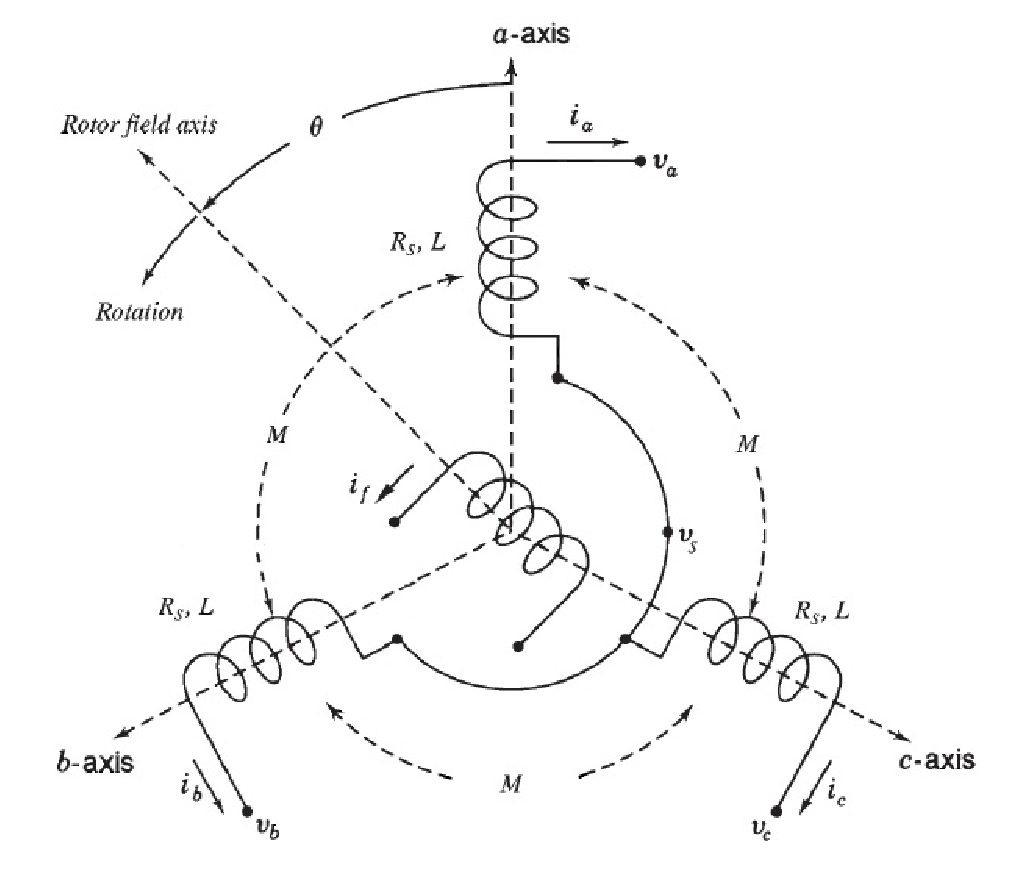
\includegraphics[scale=0.5]{SGStucture}
\par\end{centering} \label{fig:structOfSG}

\caption[Structure of an idealized three-phase round rotor synchronous
generator]{Structure of an idealized three-phase round rotor
synchronous generator, modified from \cite[Figure 3.4]{GrSt2014}.}
\end{figure}
%%%%%%%%%%**********%%%%%%%%%%**********%%%%%%%%%%**********%%%%%%%%%%

The mutual inductance between the rotor coil and each of the stator
coils varies with the rotor angle $\theta$ as follows:
$$ \left[\begin{array}{c} M_{a,f}\\ M_{b,f}\\ M_{c,f}\end{array}
   \right] \m=\m M_{f}\widetilde{\cos}\theta \m,$$
where $M_f>0$ is a constant. The vector of flux linkages of the stator
windings is
$$ \Phi \m=\m \left[\begin{array}{ccc} L & -M & -M\\ -M & L & -M\\
   -M & -M & L \end{array}\right]i + M_f i_f\widetilde{\cos}\theta
   \m.$$
Since there is no neutral line, $i_a+i_b+i_c=0$, so the previous
equation can be rewritten as 
$$\Phi \m=\m L_s i + M_f i_f \widetilde{\cos}\theta \m,$$
where $L_s=L+M$. We will assume that the rotor current is constant
(or equivalently, the rotor is composed of a permanent magnet). The
stator voltages satisfy
\BEQ{eq:SGTerminalVlotage}
   v - v^n \m=\m -R_{s}i-\frac{\dd\Phi}{\dd t} \m=\m -R_{s}i-L_{s}
   \frac{\dd i}{\dd t} + e \m,
\end{equation}
where $e=\left[e_a\ e_b\ e_c \right] ^\top$ is the back electromotive 
force (EMF) due to the rotor movement (also called synchronous 
internal voltage), given by \vspace{-2mm}
\BEQ{eq:emf}
   e \m=\m M_f i_f\dot{\theta}\widetilde{\sin}\theta \m.
\end{equation}

For a SG with no load, the voltages at each terminal
will be sinusoidal functions. In order to represent the voltages and
currents in a more convenient way, we apply the Park transformation
with respect to the rotor angle:
$$ x_{dq0} \m=\m \left[\begin{array}{c} x_{d}\\ x_{q}\\ x_{0}
   \end{array}\right] \m=\m U(\theta) \left[\begin{array}{c} x_{a}\\
   x_b\\ x_c\end{array}\right] \m=\m U(\theta) x_{abc} \m,$$
where $x_{abc}$ is a vector in $abc$ coordinates, $x_{dq0}$
is the same vector in the $dq0$ coordinates, and $U(\theta)$ is the
following unitary matrix:
\BEQ{eq:ParkTransformation}
 U(\theta) \m=\m \sqrt{\frac{3}{2}}\left[\begin{array}{ccc}
   \cos(\theta) & \cos(\theta-\frac{2\pi}{3}) & \cos(\theta-
   \frac{4\pi}{3})\\ \sin(\theta) & \sin(\theta-\frac{2\pi}{3})
   & \sin(\theta-\frac{4\pi}{3})\\ \sqrt{1/2} & \sqrt{1/2} & 
   \sqrt{1/2} \end{array}\right] \m.
\end{equation}

Applying the Park transformation to \rfb{eq:SGTerminalVlotage} 
leads to
\BEQ{aPark}
   U(\theta)(v-v^n)-U(\theta)e \m=\m -R_{s}U(\theta)i - L_s 
   U(\theta) \frac{\dd i}{\dd t} \m.
\end{equation}
Now we use that, denoting $i_{dq0}=U(\theta)i$,
$$ \frac{\dd i_{dq0}}{\dd\theta} \m=\m U(\theta)\frac{\dd i}
   {\dd\theta} + \frac{\dd U(\theta)}{\dd\theta}i \m=\m
   U(\theta)\frac{\dd i}{\dd\theta} + \left[\begin{array}{c}
   i_{q}\\ -i_{d}\\ 0 \end{array}\right].$$
This implies that \vspace{-2mm}
$$ \dot{i}_{dq0} \m=\m \frac{\dd i_{dq0}}{\dd\theta} \cdot \frac
   {\dd\theta}{\dd t} \m=\m U(\theta)\dot{i} + \o\left[\begin{array}
   {c} i_q\\ -i_d\\ 0 \end{array}\right] \m,$$
where $\o=\dot{\theta}$. We rewrite \rfb{aPark} as follows:
\BEQ{eq:idiqDynamics}
   L_s\frac{\dd}{\dd t}\nm\left[\nm\begin{array}{c} i_d\\ i_q\\ i_0
   \end{array}\nm\right] - L_s \o \left[\nm\begin{array}{c} i_q\\ -i_d
   \\ 0 \end{array}\nm\right] = -R_s\left[\begin{array}{c} i_d\\
   i_q\\ i_0 \end{array}\right] + \left[\nm \begin{array}{c} e_d-v_d
   \\ e_q-v_q\\ \tilde v\end{array}\nm\right],
\end{equation}
where $\tilde v=e_0-v_0+v^n_0$. Here we have used that (obviously)
$v^n_d=v^n_q=0$. Since there is no neutral connection, $i_0=0$, hence
$\tilde v=0$. Applying the Park transformation to \rfb{eq:emf} gives
$$ \left[\begin{array}{c} e_d\\ e_q \end{array}\right] \m=\m -\sqrt
   {\frac{3}{2}} M_{f} \left[ \begin{array}{c} 0\\ \o i_f
   \end{array}\right] \m.$$
We denote $m=\sqrt{\frac{3}{2}}M_{f}$. If we substitute the last
formula into \rfb{eq:idiqDynamics}, we get
\BEQ{eq:idiqDynamicsWithExIf}
   L_s\frac{\dd}{\dd t} \nm \left[\nm \begin{array}{c}
   i_d\\ i_q \end{array} \nm\right] = -R_s\left[\nm \begin{array}{c}
   i_d\\ i_q \end{array} \nm\right]+\o L_s\left[\nm\nm \begin{array}
   {c} i_q\\ -i_d\end{array} \nm\nm\right]\\ -m\left[\nm\nm 
   \begin{array}{c} 0\\ \o i_f\end{array} \nm\nm\right] - \left[\nm 
   \begin{array}{c} v_d\\ v_q \end{array} \nm\right] .
\end{equation}

The rotational dynamics of the rotor is given by
\BEQ{eq:mechanicalPart}
   J\dot{\omega} \m=\m T_{m}-T_{e}-D_{p} \omega \m,
\end{equation}
where $J$ is the moment of inertia of the rotor, $T_m-D_p\o$ is is the
mechanical torque coming from the prime mover, $T_e$ is the
electromagnetic torque developed by the generator, and $D_p$ is a the
frequency droop coefficient. The feedback term $D_p\o$ is used in
order to control the frequency of the grid, see \cite{Kundur},
\cite{PoDoBu:13}, \cite{CaTa:14}, \cite{ZhWe:11}. $T_e$ can be found
using energy consideration. It is easy to see that the magnetic 
energy stored in the generator is
$$ E_{mag} \m=\m \half \left(\langle i,L_s i \rangle + L_f i_f^2
   \right) + M_f i_f \langle i,\widetilde{\cos}\theta \rangle \m.$$
The electromagnetic torque can be calculated as follows:
$$ T_e \m=\m \frac{\partial E_{mag}}{\partial\theta}|_{\Phi,\Phi_f
   \ const.} \m=\m - \frac{\partial E_{mag}}{\partial\theta}|_{i,
   i_f\ const.}$$
(see \cite{ZhWe:11}), whence
$$ T_e \m=\m M_f i_f \left\langle i,\frac{\dd\tilde{\cos}\theta}
   {\dd\theta} \right\rangle \m=\m M_f i_f \langle i,\widetilde
   {\sin} \theta\rangle \m=\m -m i_f i_q \m.$$
Using \rfb{eq:idiqDynamicsWithExIf}, \rfb{eq:mechanicalPart}
and the last formula, we obtain
\BEQ{eq:SingleSGDynamics}
   \frac{\dd}{\dd t}\nm\left[\nm \begin{array}{c} L_s i_d\\ L_s i_q\\ 
   J\o\end{array} \nm\right] = \left[\nm \begin{array}{ccc} -R_s & 
   \o L_s & 0\\ -\o L_s & -R_s & -mi_f\\ 0 & mi_f & -D_p \end{array}
   \nm\right] \nm \left[\nm \begin{array}{c} i_d\\ i_q\\ \o 
   \end{array} \nm\right] + \left[\nm\nm \begin{array}{c} -v_d\\ -v_q
   \\ T_m \end{array} \nm\nm\right].
\end{equation}
This third order nonlinear dynamical system represents the dynamics
of a single SG with constant field current, if we ignore the rotor 
angle $\theta$. 

\section{TICSG modeling}

In this section we develop a model for a microgid comprising of two identical SGs connected in parallel with a resistive load, assuming constant field current (see Figure \ref{fig:TICSGThreePhase}).

%%%% Figure Tree phase TICSG system.
\begin{figure}[!htb]
\begin{circuitikz}[american voltages,scale=0.6, transform shape]
\begin{scope}[shift={(-5,0)}]     \draw (0,0) node[anchor=east] {0} to [L=Z, *-o] (90 :2.5) node[anchor=east]{$v_a$}; \draw (0,0) to [L=Z, *-o] (210 :2.5) node[anchor=east]{$v_b$}; \draw (0,0) to [L=Z, *-o] (330 :2.5) node[anchor=east]{$v_c$}; \node (0,0) [align=left,text width=4cm] {SG1}; \end{scope}
   \draw (0,0) node[anchor=east] {0} to [R=$R_L$, *-o] (90 :2.5) node[anchor=east]{}; \draw (0,0) to [R=$R_L$] (210 :2.5); \draw (0,0) to [R=$R_L$] (330 :2.5);
\begin{scope}[shift={(5,0)}]    \draw (0,0) node[anchor=east] {0} to [L=Z, *-o] (90 :2.5) node[anchor=west] {$v_a$}; \draw (0,0) to [L=Z, *-o] (210 :2.5) node[anchor=east]{$v_b$}; \draw (0,0) to [L=Z, *-o] (330 :2.5) node[anchor=east]{$v_c$}; \node (0,0) [align=left,text width=4cm] {SG2}; \end{scope}
\draw (5,2.5) to [short, i>=$i_{a2}$] (0,2.5) to [short, i<=$i_{a1}$] (-5,2.5); \draw (-2.165 +5,-1.25) to [short] (-2.165 +5,-1.25 -1) to [short, i>=$i_{b2}$]   (-2.165 ,-1.25-1)  to [short, o-] (-2.165 ,-1.25 ); \draw (-2.165 -5,-1.25) to [short] (-2.165 -5,-1.25 -1) to [short, i>=$i_{b1}$]   (-2.165 ,-1.25-1); \draw (2.165 +5,-1.25) to [short] (2.165 +5,-1.25 -2) to [short, i>=$i_{c2}$]  (2.165 ,-1.25-2)  to [short, o-] (2.165 ,-1.25 ); \draw (2.165 -5,-1.25) to [short] (2.165 -5,-1.25 -2) to [short, i>=$i_{c1}$]  (2.165 ,-1.25-2);
\end{circuitikz}\caption{{\em two identical coupled SGs} (TICSG) model - three phase diagram}

\label{fig:TICSGThreePhase}
\end{figure}

%%%%%%%%%%%%%
We denote the first SG rotor angle as  $\theta_{1}$ and the second SG rotor angle as $\theta_{2}$. We assume identical constant torque that act on each of the generators, denoted as $T_{m}$. By symmetry,
we assume that the voltages at the (non-connected) midpoints of the
generators and the load are zero.

We denoted the phase voltages and currents of the first generator as: $v_{1}=\left[v_{a1}\  v_{b1}\  v_{c1}
\right]^\top$ and $i_{1}=\left[i_{a1}\  i_{b1}\  i_{c1}
\right]^\top$  respectively.
Similarly, we denoted the phase voltages and currents of the second generator as: $v_{2}=\left[v_{a2}\  v_{b2}\  v_{c2}
\right]^\top$ and $i_{2}=\left[i_{a2}\  i_{b2}\  i_{c2}
\right]^\top$ respectively.

We denote by $Z$ the impedance of each SG stator. This impedance is comprised by the resistive impedance of the stator coil $R_s$ and the inductive impedance of the stator, namely $Z\left(s\right)=R_{s} + sL_{s}$. In general, the line that connects the SG to the grid has its impedance that can be modeled (in most cases) as a resistance and an inductance in series, but these values can simply be added to the parameters $R_s$ and $L_s$ of the SG.
One phase scheme of the grid is presented at Figure \ref{fig:TICSGOnePhase}.


%%%% Figure Tree phase TICSG system.
\begin{figure}[!htb]
\begin{circuitikz}[american voltages,scale=0.6, transform shape]
\draw   (0,0) node[ground] {}   to [V,v=$e_{j1}$] (0,3) {}   to [R=$R_s$,i>=$i_{j1}$] (3,3){}   to [L=$L_s$] (5,3){}   to [R=$R_L$, o-] (5,0){}    to  (5,0) node[ground] {};   \draw   (10,0) node[ground] {}   to [V,v=$e_{j2}$] (10,3) {}   to [R=$R_s$,i>=$i_{j2}$] (7,3){}   to [L=$L_s$] (5,3){};   \node[draw] at (-1,4) {$j \in \{a,b,c\}$}; \end{circuitikz} 

\caption{{\em two identical coupled SGs} (TICSG) model - one phase diagram}

\label{fig:TICSGOnePhase}
\end{figure}

%%%%%%%%%

In order to use the four order model of single SG \eqref{eq:SingleSGDynamics} in this system, we apply  Park transformation \eqref{eq:ParkTransformation}, on the voltages: $\left[ v_{di}\ v_{qi}\  v_{0i} \right]^\top=U(\theta_{i})\left[v_{ai}\ v_{bi}\ v_{ci}  \right]^\top$,  and currents $\left[v_{di}\ v_{qi}\  v_{0i} \right]^\top=U(\theta_{i})\left[v_{ai}\ v_{bi}\ v_{ci}  \right]^\top$ where $i \in \{1,2\}$.

From Kirchhoff's laws $i_{01}=i_{02}=0$ () and by symmetry
argument we can see that $v_{01}=v_{02}=0$.

Thus, we only have to deal with $v_{dj},v_{qj}$ (with $j\in\{1,2\}$). 

We denote 
$$\delta=\theta_{2}-\theta_{1}$$

The voltage of the load is:
$$v_L=R_{L}(i_{1}+i_{2})$$

Rewriting this equation and after applying Park transformation yields,
for the first SG:
$$
\left[\begin{array}{c}
v_{d1}\\
v_{q1}\\
0
\end{array}\right]=R_{L}\left[\begin{array}{c}
i_{d1}\\
i_{q1}\\
0
\end{array}\right]+R_{L}U(\theta_{1})\left[\begin{array}{c}
i_{a2}\\
i_{b2}\\
i_{c2}
\end{array}\right]
$$

Note, that $U(\theta_{1})\left[ i_{a2}\ i_{b2}\ i_{c2}\right]^\top \neq \left[ i_{d2}\ i_{q2}\ i_{02}\right]$ because the  Park transformations depends on  $\theta_1$ instead of $\theta_2$. 

We express  the currents of the second SG in the d-q coordinates by using the inverse Park transformation: 
\BEQ{eq:TICSGVolAndCurr}
 \left[\begin{array}{c}
v_{d1}\\
v_{q1}\\
0
\end{array}\right]=R_{L}\left[\begin{array}{c}
i_{d1}\\
i_{q1}\\
0
\end{array}\right]+R_{L}U(\theta_{1})U(\theta_{2})^{-1}\left[\begin{array}{c}
i_{d2}\\
i_{q2}\\
0
\end{array}\right].
\end{equation}

A simple computation shows that 
\BEQ{eq:ParkChangeAngle}
  U(\theta_{1})U(\theta_{2})^{-1}=\left[\begin{array}{ccc}
\cos(\delta) & -\sin(\delta) & 0\\
\sin(\delta) & \cos(\delta) & 0\\
0 & 0 & 1
\end{array}\right].
\end{equation}

(recall that $\delta=\theta_{2}-\theta_{1}$).

Substitute \eqref{eq:SingleSGDynamics} and \eqref{eq:ParkChangeAngle} into \eqref{eq:TICSGVolAndCurr}  gives:

\[
\varLambda\dot{z}_{1}=\mathcal{A}(\omega_{1})z_{1}+T_{m}e_{3}-\mathcal{B}(\delta)z_{2}
\]
Where denoting
 \[z_{i}=\left[i_{di}\ i_{qi}\  \omega_{i}\right]^\top,i\in\{1,2\}\]

\[
\varLambda=\left[\begin{array}{ccc}
L_{s} & 0 & 0\\
0 & L_{s} & 0\\
0 & 0 & J
\end{array}\right]
\]

\[
\mathcal{A}(\omega)=\left[\begin{array}{ccc}
-R_{tot} & \omega L_{s} & 0\\
-\omega L_{s} & -R_{tot} & -mi_{f}\\
0 & mi_{f} & D_{p}
\end{array}\right]
\]
\[\mathcal{B}(\delta)=\left[\begin{array}{ccc}
R_{L}\cos(\delta) & -R_{L}\sin(\delta) & 0\\
R_{L}\sin(\delta) & R_{L}\cos(\delta) & 0\\
0 & 0 & 0
\end{array}\right]
\]
\[e_{3}=\left[0\ 0\ 1\right]^\top\]
\[ R_{tot}=R_{s}+R_{L} \]

Of course a symmetric equation holds for the second generator:

\[
\varLambda\dot{z}_{2}=\mathcal{A}(\omega_{2})z_{2}+T_{m}e_{3}-\mathcal{B}(-\delta)z_{1}
\]

There is a seventh state variable, $\delta$, for which the ODE is 

\[
\dot{\delta}=\omega_{2}-\omega_{1}
\]

The whole system is described by:

\begin{equation}
\begin{array}{ccc}
\frac{d}{dt}\left[\begin{array}{c}
\varLambda z_{1}\\
\varLambda z_{2}\\
\delta
\end{array}\right] & = & \left[\begin{array}{c|c|c}
\mathcal{A}(\omega_{1}) & -\mathcal{B}(\delta) & 0\\
\hline -\mathcal{B}(-\delta) & \mathcal{A}(\omega_{2}) & 0\\
\hline -e_{3}^{T} & e_{3}^{T} & 0
\end{array}\right]\left[\begin{array}{c}
z_{1}\\
z_{2}\\
\delta
\end{array}\right]\\
 &  & +T_{m}\left[\begin{array}{c}
e_{3}\\
e_{3}\\
0
\end{array}\right]
\end{array}\label{eq:TICSGDynamics}
\end{equation}

%%%%%%%%%%**********%%%%%%%%%%**********%%%%%%%%%%**********%%%%%%%%%%
\section{The improved swing equation}

In this section, we show the relation between the ISE and the FOM. We
start with the FOM, and by a model reduction process, we get the ISE
model.  We apply ideas from singular perturbation analysis (see for
instance \cite{Khalil}). The FOM \rfb{eq:SGDynamicsInfBus} has the
following structure: \vspace{-2mm}
$$\Lambda \m \dot{z} \m=\m F(z) \m,$$ 
where $\Lambda$ is a diagonal $4\times 4$ matrix with positive
coefficients on the diagonal. Because the first two coefficients on
the diagonal of $\Lambda$ are equal to $L_s$, which in some sense can
be regarded as being small, we rewrite this dynamical system in the
following form:
$$ \left\{ \begin{array}{c} \dot{x} \m=\m f(x,y,\e) \m,\\
   \e\dot{y} \m=\m g(x,y,\e) \m. \end{array}\right.$$
By doing this, we have separated the state variables into a vector of 
fast variables, denoted by $y$, and another of slow variables, denoted
by $x$. Here, $\e>0$ is the small parameter.

We assuming that $\e$ is very small, meaning that for each $x$, the 
vector $y$ converges to a temporary equilibrium value (that depends on
$x$) much faster than the rate of change of $x$. In our specific case,
$\e=L_s$, $x=\left[\begin{array}{c} \o\\ \delta\end{array}\right]$ and
$y=\left[\begin{array}{c} i_d\\ i_q \end{array}\right]$. By taking the
first and second lines from \rfb{eq:SGDynamicsInfBus}, we have
$$ g(x,y,\e) \m=\m \left[\nm \begin{array}{cc} -R_s & \o L_s\\ -\o 
   L_s & -R_s \end{array}\nm\right] \left[\nm \begin{array}{c} i_d\\ 
   \i_q \end{array} \nm\right]+\left[\begin{array}{c} V\sin\delta\\ 
   V\cos\delta - mi_f\o \end{array}\right].$$
Our assumption that $\e$ is very small means that the subsystem $\e
\dot{y}=g(x,y,\e)$ is much faster than $\dot{x}=f(x,y,\e)$ and it is 
also stable, so that it will reach its temporary equilibrium almost 
instantly compared to the slow movement of $x$. The temporary 
equilibrium point $\hat{y}(x,\e)$ is the solution of $g(x,\hat y,\e)=
0$. The solution of this linear equation (in $\hat{y}$) is
$$ \hat{y} \m=\m -\left[\begin{array}{cc} -R_s & \o L_s\\
   -\o L_s & -R_s \end{array}\right]^{-1}\left[\begin{array}{cc}
   V\sin\delta\\ V\cos\delta - mi_f\o \end{array}\right]$$
$$ \m\qquad=\m \left[\begin{array}{cc} \frac{R_s V\sin\delta - L_s\o
   \left(mi_f\o - V\cos\delta\right)}{L_s^{2}\o^2+R_s^2}\\
   \frac{-R_s\left(mi_f\o - V\cos\delta\right) - L_s V\o\sin\delta}
   {L_s^2\o^2 + R_s^2} \end{array}\right] \m.$$
Assuming that $R_s$ is small so that the terms containing $R_s$ are
negligible, we obtain the following approximation of $\hat y$:
\BEQ{eq:ISEInfBusEstimatedCurrents}
   \hat{y}_{app} \m=\m \left[\begin{array}{c} \hat{i}_d\\
   \hat{i}_q \end{array}\right] \m=\m \left[\begin{array}{c}
   \frac{V\cos\delta - mi_f\o}{L_s\o}\\ -\frac{V\sin\delta}{L_s\o}
   \end{array}\right] \m.
\end{equation}

We substitute $\hat{y}_{app}$ obtained above into $\dot{x}=f(x,y,\e)$
(in place of $y$) to get the reduced model
$$ \left\{ \begin{array}{c} J\dot{\o}\o+D_p\o^2 \m=\m -\frac{mi_f V
   \sin\delta}{L_s}+T_m\o \m,\\ \dot{\delta} \m=\m \o-\o_g \m.
   \end{array}\right.$$
The power absorbed from the prime mover can be expressed approximately
(assuming constant torque) as
$$P_m \m=\m (T_m-D_p \o_g)\o \m.$$
If we express from here $T_m\o$ and substitute into the model 
derived a little earlier, we obtain
$$ \left\{ \begin{array}{c} J\dot{\o}\o+D_p\o(\o-\o_g) \m=\m P_m - 
   \frac{mi_f V\sin\delta}{L_s} \m,\\ \dot{\delta} \m=\m \o-\o_g \m.
   \end{array}\right.$$
This model is known as the {\em improved swing equation} (ISE) model,
see \cite{DePersiSchaft:16}, \cite{ZhouOhsawa2009}. Note that we did 
many different approximations to derive it.

%%%%%%%%%%**********%%%%%%%%%%**********%%%%%%%%%%**********%%%%%%%%%%
\section{Simulations}

In this section we present simulations which demonstrate that the ISE
model is a good approximate model in many cases. We also show that
there are cases in which there is a significant mismatch between the
behavior suggested by the ISE model and the FOM. In each simulation
result, the behavior of $i_d$ and $i_q$ over time is described for
both the FOM and the ISE models. Note that for the ISE model, we use
\eqref{eq:ISEInfBusEstimatedCurrents} to estimate these currents. We 
plot the frequency $\o$ and the power angle $\delta$ as functions of
time for these two models.

\subsection{5KW SG}

%%%%%%%%%%**********%%%%%%%%%%**********%%%%%%%%%%**********%%%%%%%%%%
\begin{figure}[ht]
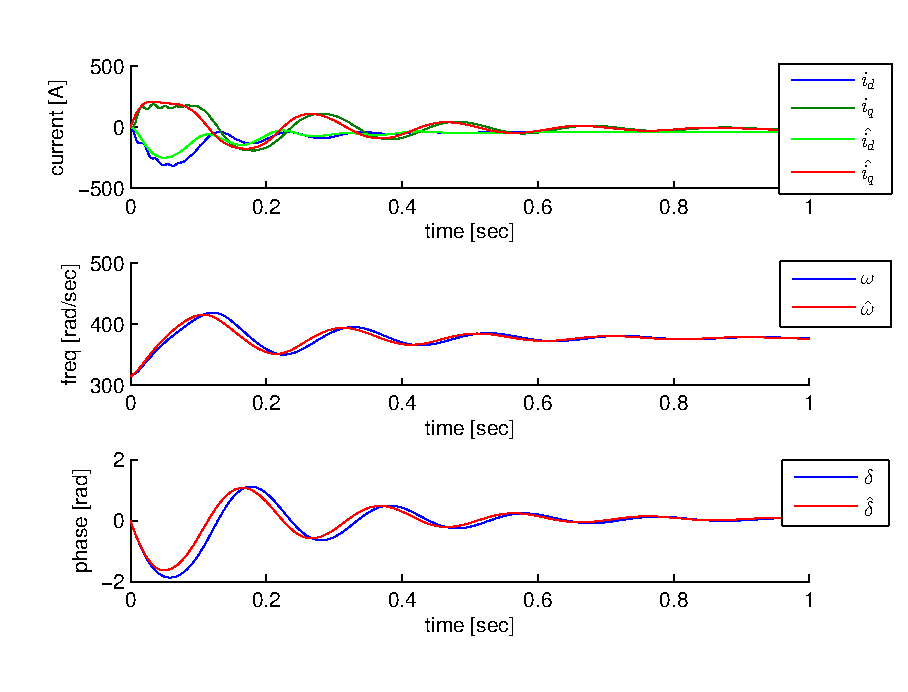
\includegraphics[scale=0.6]{sim5KWInfBus}

\caption{Simulations for a 5KW SG onnected to an infinite bus,
using both models. For $\o$ and $\delta$ the results are very 
similar.} \label{fig:InfBusOne5KWSG}
\end{figure}
%%%%%%%%%%**********%%%%%%%%%%**********%%%%%%%%%%**********%%%%%%%%%%


As shown in Figure \ref{fig:InfBusOne5KWSG}, simulations indicates
that for the 5KW SG, the behavior of the FOM and the ISE is almost the
same. Although the currents at the reduced don't have a ripple that
the FOM has, both models converge at the same rate with the same
oscillations to the same equilibrium point (The parameters for this
simulation are $J=0.2$ {[}$kgm^{2}${]}, $D_{p}=1.7$ {[}$J/sec${]},
$R_{s}=0.152$ {[}$\Omega]$, $L_{s}=4.4$ {[}$mH${]}, $mi_{f}=1.05$
{[}$Vsec]$, $\omega_{g}=60\cdotp2\pi$ {[}$rad/sec${]}, $V=330$
{[}$V]$, $Pm=5$ {[}$kW${]}).

\subsection{1MW SG}

%%%%%%%%%%**********%%%%%%%%%%**********%%%%%%%%%%**********%%%%%%%%%%
\begin{figure}[ht]
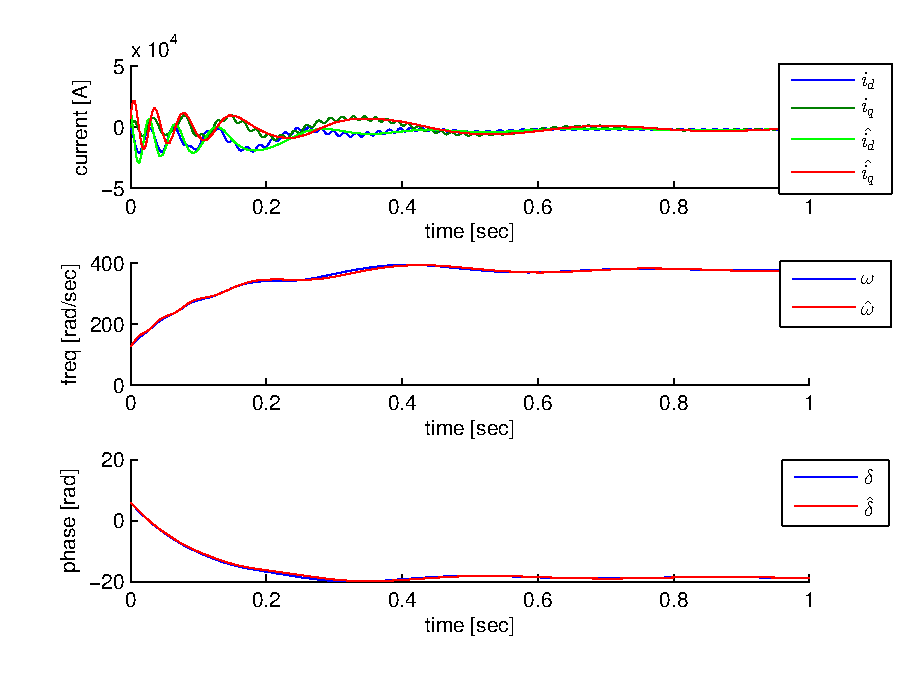
\includegraphics[scale=0.6]{sim1MWInfBus}

\caption{Simulation for a 1MW SG on an infinite bus, both models}
\label{fig:InfBusOne1MWSG}
\end{figure}
%%%%%%%%%%**********%%%%%%%%%%**********%%%%%%%%%%**********%%%%%%%%%%

As shown in Figure \ref{fig:InfBusOne1MWSG}, simulations show that
for the 1MW SG, the behavior of the FOM and the ISE are still very similar. Although the FOM currents
are much more rippled than the ISE currents, both models converge
at the same rate with the same oscillations to the same equilibrium
point (The parameters for this simulation are $J=40.05$ {[}$kgm^{2}${]},
$D_{p}=337$ {[}$J/sec${]}, $R_{s}=0.4$ {[}$\Omega]$, $L_{s}=18$
{[}$mH${]}, $mi_{f}=1.79$ {[}$Vsec]$, $\omega_{g}=60\cdotp2\pi$
{[}$rad/sec${]}, $V=563$ {[}$V]$, $Pm=1$ {[}$MW${]}). 

\subsection{Non stable behavior of the reduced model}

%%%%%%%%%%**********%%%%%%%%%%**********%%%%%%%%%%**********%%%%%%%%%%
\begin{figure}[ht]
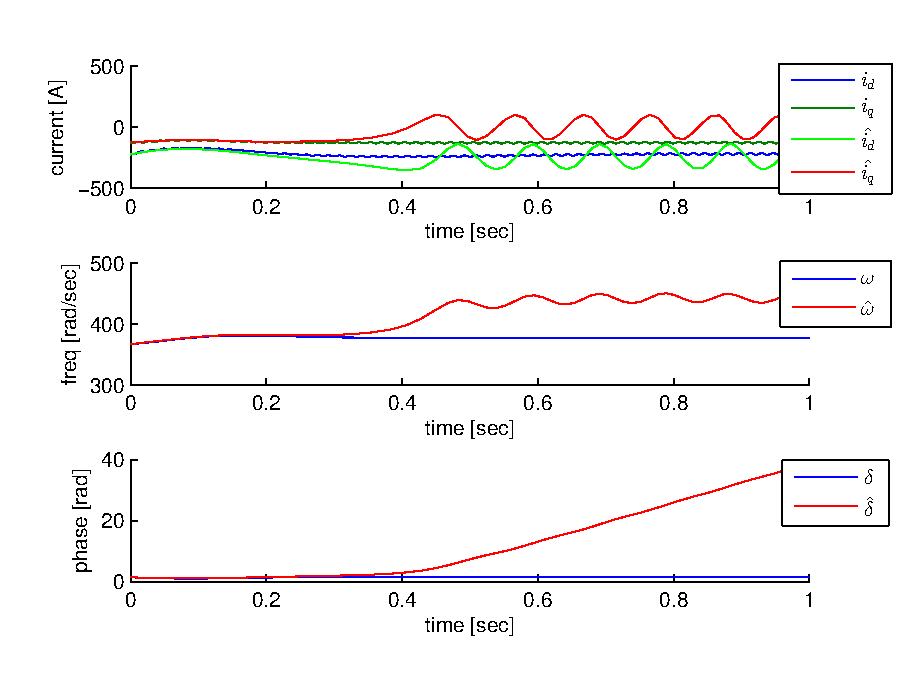
\includegraphics[scale=0.6]{simDiffBehavior1}

\caption{A simulation example showing different behavior for the 
         FOM and the ISE reduced model for a 50 KW SG}
\label{fig:InfBusOne1DiffBehavior1}
\end{figure}
%%%%%%%%%%**********%%%%%%%%%%**********%%%%%%%%%%**********%%%%%%%%%%

As shown in Figure \ref{fig:InfBusOne1DiffBehavior1}, simulations
show that for other parameters set (the parameters for this simulation
are $J=0.2$ {[}$kgm^{2}${]}, $D_{p}=1.7$ {[}$J/sec${]}, $R_{s}=0.152$
{[}$\Omega]$, $L_{s}=4.4$ {[}$mH${]}, $mi_{f}=1.05$ {[}$Vsec]$,
$\o_g=60\cdotp2\pi$ {[}$rad/sec${]}, $V=200$ {[}$V]$, $P_m=50$
{[}$KW${]}) the behavior of the FOM and the ISE is significantly 
different. While the fourth order model is stable
(the eigenvalues of the Jacobian around the equilibrium point are:
$$\left[-11.41+376.9i,-11.41-376.9i,-508+837i,-508-837i\right]$$
the reduced model is not stable (the eigenvalues of the Jacobian
around the equilibrium point are: 
$\left[-14.6+9.4979i,\:6.1-9.4i\right]$).

%%%%%%%%%%**********%%%%%%%%%%**********%%%%%%%%%%**********%%%%%%%%%%
\subsection{An example for different region of attraction}

\begin{figure}[ht]
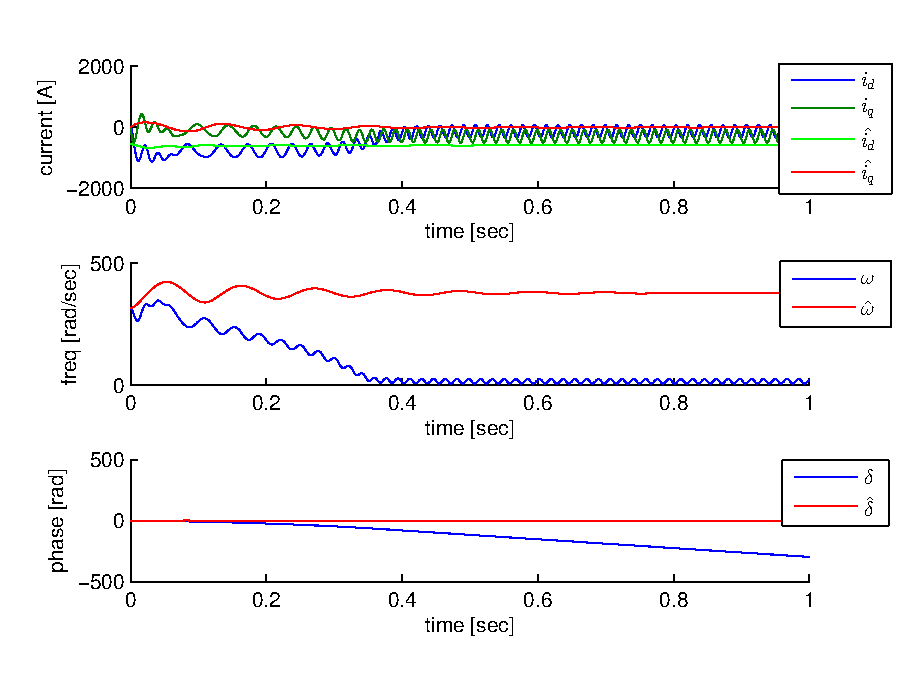
\includegraphics[scale=0.6]{simDiffRegionOFAttraction}
\caption{Simulation example that shows different behavior for the 
full and the reduced models, for a 5 KW SG.}
\label{fig:InfBusOne1DiffRegionOfAttraction}
\end{figure}

As shown in Figure \ref{fig:InfBusOne1DiffRegionOfAttraction},
simulations show that for some parameters set (The parameters for this
simulation are $J=0.2$ {[}$kgm^{2}${]}, $D_{p}=1.7$ {[}$J/sec${]},
$R_{s}=0.152$ {[}$\Omega]$, $L_{s}=1.05$ {[}$mH${]}, $mi_{f}=3.5$
{[}$Vsec]$, $\omega_{g}=60\cdotp2\pi$ {[}$rad/sec${]}, $V=330$
{[}$V]$, $P_m=5$ {[}$KW${]}) the initial condition of this simulation
is within the region of attraction of the reduced model, but outside
the region of attraction of the FOM. That cause the FOM to diverge while the ISE converges to the
equilibrium point.

%%%%%%%%%%++++++++++%%%%%%%%%%++++++++++%%%%%%%%%%++++++++++%%%%%%%%%%
\section{Conclusions}

We have investigated the relation between the FOM of a SG with constant
field current connected to an infinite bus and the reduced ISE model. 
Simulations show that sometimes the FOM shows a behavior which does
not match the one suggested by the ISE model. 

%%%%%%%%%%++++++++++%%%%%%%%%%++++++++++%%%%%%%%%%++++++++++%%%%%%%%%%
\begin{thebibliography}{10}

\bibitem{Kundur} P.~Kundur, \emph{Power System Stability and Control}.
 \hskip 1em plus 0.5em minus 0.4em\relax McGraw-Hill, New York, 1994.

\bibitem{GrSt2014} J.J.~Grainger and W.D.~Stevenson,
 {\em Power Systems Analysis}, \m McGraw-Hill, New York, 1994.

\bibitem{SauerPai1998} P.~W.~Sauer and M.~A.~Pai, \m {\em Power 
 Systems Dynamics and Stability}, Stipes Publishing, Champaign,
 IL, 1997.

\bibitem{GOBS:03}
 M.~Galaz, R.~Ortega, A.S.~Bazanella and A.M.~Stankovic, \m
 An energy-shaping approach to the design of excitation control
 of synchronous generators, {\em Automatica}, vol.~39, 2003,
 pp.~111-119.

\bibitem{DoBull:12} F. D{\"o}rfler and F. Bullo, \m 
 \emph{Synchronization and transient stability in power networks and
 nonuniform Kuramoto oscillators}.\hskip 1em plus 0.5em minus 
 0.4em\relax SIAM J. Control and Optim., vol.~50, 2012, 
 pp.~1616-1642.

\bibitem{PoDoBu:13} J.W.~Simpson-Porco, F.~D{\"o}rfler
 and F.~Bullo, \m Synchronization and power sharing for
 droop-controlled inverters in islanded microgrids, {\em 
 Automatica}, vol. 49, 2013, pp.~2603-2611.

\bibitem{CaTa:14} S.Y.~Caliskan and P.~Tabuada, \m
 Compositional transient stability analysis of multimachine 
 power networks, {\em IEEE Trans. Control of Network Systems}, 
 vol.~1, 2014, pp.~4-14.

\bibitem{NaWe:14} V.~Natarajan and G.~Weiss, \m Almost global 
 asymptotic stability of a constant field current synchronous 
 machine connected to an infinite bus, {\em Proc. of the 53rd 
 IEEE Conf. on Decision and Control}, Los Angeles, CA, Dec. 2014, 
 pp.~3272-3279.

\bibitem{NaWe:15} V.~Natarajan and G.~Weiss, \m Almost global 
 asymptotic stability of a grid-connected synchronous generator,
 submitted in 2015.

\bibitem{DePersiSchaft:16} P.~Monshizadeh, C.~De Persis,
 N.~Monshizadeh and A.~van der Schaft, \m Nonlinear Analysis
 of an improved wwing equation, \m submitted in 2016.

\bibitem{Walker:94} J.H.~Walker, \m {\em Large Synchronous Machines: 
 Design, Manufacture and Operation}, \m Oxford University Press, 
 Oxford, 1981.

\bibitem{Fitzgerald:03} A.E.~Fitzgerald, C.~Kingsley and S.D.~Umans,
 \m {\em Electric Machinery}, \m McGraw-Hill, New York, 2003.

\bibitem{MaWe:15} Y.~Mandel and G.~Weiss, \m Adaptive internal model
 based suppression of torque ripple in brushless DC motor drives,
 {\em Systems Science \& Control Engineering}, vol.~5, 2015, 
 pp.~162-176.

\bibitem{Khalil} H.K.~Khalil, \m \emph{Nonlinear Systems} (third 
 edition), Prentice Hall, New Jersey, 2002.

\bibitem{ZhWe:11} Q.-C.~Zhong and G.~Weiss, \m Synchronverters: 
 Inverters that mimic synchronous generators, {\em IEEE Trans. 
 Industr. Electronics}, vol.~58, 2011, pp.~1259-1267.

\bibitem{ZhouOhsawa2009} J.~Zhou and Y.~Ohsawa, \m Improved swing
 equation and its properties in synchronous generators, {\em
 IEEE Trans. Circuits and Systems I}, vol.~56, 2009, pp.~200-209.

\end{thebibliography}
\end{document}
